\subsection{Fonction de Hurst}

\begin{minipage}{0.47\linewidth}
	On appelle $H : t \mapsto H_t$ la fonction de Hurst, celle qui a été choisie est la suivante :

	$$
		H^{[0.4, 0.8, 5, 0.5]}_{\textsf{logistic}} : \begin{array}{ccc}
			[0,1] & \longrightarrow & [0.4, 0.8]
			\\
			t     & \longmapsto     & 0.4 + \frac{(0.8 - 0.4)}{1 + e^{-5(t - 0.5)}}
		\end{array}
	$$

	On dispose donc d'une régularité locale qui varie sur $\mathcal T$, tout en ayant une évolution pas trop brusque. Nous allons étudier le comportement du $\Delta$ lors de l'estimation de la régularité locale en les points suivants :

	$$
		\vec t = \begin{bmatrix} 0.3 \\ 0.4 \\ 0.5 \\ 0.6 \\ 0.7 \\ 0.8 \end{bmatrix}
		\quad\quad
		H(\, \vec t \,) =
		\begin{bmatrix}
			0.51 \\ 0.55 \\ 0.6 \\ 0.65 \\ 0.69 \\ 0.73
		\end{bmatrix}
	$$

\end{minipage}
\hfill
\begin{minipage}{0.47\linewidth}
	\begin{figure}[H]
		\centering
		\begin{tikzpicture}
			\begin{axis}[
					width=\textwidth,
					xlabel=$t$,
					ylabel={$H^{[0.4, 0.8, 5, 0.5]}_{\textsf{logistic}}(t)$},
					xmin=0, xmax=1,
					ymin=0.4, ymax=0.8,
					axis lines=center,
					axis on top=true,
					domain=0:1,
					samples=100,
					legend style={at={(0.5,-0.15)},anchor=north},
					legend entries={Fonction de Hurst, Points d'estimation de la régularité locale},
				]
				\addplot [mark=none,smooth,blue] {0.4 + (0.8 - 0.4)/(1 + exp(-5*(x - 0.5)))};
				\addplot [only marks,mark=*] coordinates {
						(0.3,0.51)
						(0.4,0.55)
						(0.5,0.6)
						(0.6,0.65)
						(0.7,0.69)
						(0.8,0.73)
					};
			\end{axis}
		\end{tikzpicture}
		\caption{Hurst Function : Logistic}
		\label{plot:hurst-logistic}
	\end{figure}
\end{minipage}


\subsection{Constante de Hölder
}

$$\forall t \quad L_t = 1$$


\subsection{Moyenne}


\begin{minipage}{0.47\linewidth}

	La fonction moyenne du processus que l'on souhaite retrouver après bruitage est la suivante :

	$$
		\mu : \begin{array}{ccc}
			[0,1] & \longrightarrow & \mathbb R
			\\
			t     & \longmapsto     & 4 \cdot \sin\bigl( \frac 3 2 \pi \cdot t \bigr)
		\end{array}
	$$
\end{minipage}
\hfill
\begin{minipage}{0.47\linewidth}
	\begin{figure}[H]
		\centering
		\begin{tikzpicture}
			\begin{axis}[
					width = \textwidth,
					xlabel=$t$,
					ylabel=$\mu(t)$,
					xmin=0, xmax=1,
					ymin=-4, ymax=4,
					axis lines=center,
					axis on top=true,
					domain=0:1,
					samples=100
				]
				\addplot [mark=none,smooth,blue] {4*sin(deg(3/2*pi*x))};
			\end{axis}
		\end{tikzpicture}
		%\caption{Mean function : $\mu(t) = 4 \cdot \sin\bigl( \frac 3 2 \pi \cdot t \bigr)$}
		\label{plot:mu}
	\end{figure}
\end{minipage}







\subsection{Noyau de la relation FAR(1)}
\begin{minipage}{0.48\linewidth}
	On décide de simuler un FAR(1) basé sur un opérateur linéaire intégral :

	$$
		X_{n+1} = \phi(X_n) + \varepsilon_{n+1}
	$$

	avec : $\phi : f \mapsto \displaystyle\int_{\mathcal T} f(u) \beta(u, \cdot \,) \, du$

	C'est une modélisation fréquente des FAR(1). Le noyaux que l'on considère dans l'opérateur intégral pour les simulations est le suivant :


	$$
		\beta : \, \begin{array}{ccc}
			[0,1]^2 & \longrightarrow & \mathbb R
			\\
			(t,s)   & \longmapsto     & \frac 9 4 t\sqrt{ s(1-s) }
		\end{array}
	$$

\end{minipage}
\hfill
\begin{minipage}{0.48\linewidth}
	\begin{figure}[H]
		\centering
		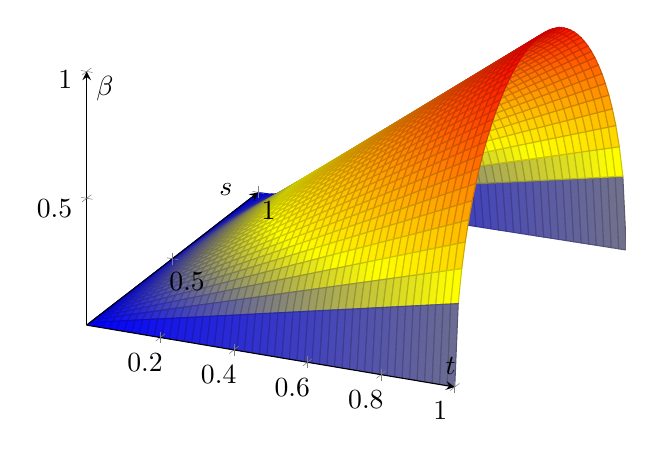
\begin{tikzpicture}
			\begin{axis}[
					xlabel=$t$,
					ylabel=$s$,
					zlabel=$\beta$,
					xmin=0, xmax=1,
					ymin=0, ymax=1,
					zmin=0, zmax=1,
					axis lines=center,
					axis on top=true,
					domain=0:1,
					samples=50,
				]
				\addplot3 [surf] {9/4*x*sqrt(y*(1-y))};
			\end{axis}
		\end{tikzpicture}
		\caption{Graphique du noyau intégral pour la relation FAR(1)}
		\label{graph:far_kernel}
	\end{figure}
\end{minipage}

on notera que le noyaux utilisé pour la relation de FAR(1) est une fonction lisse. \editorwarn{il me semble qu'il est important que le noyaux soit plus régulier que le processus, mais c'est à vérifier}

\subsection{Nombre de courbes}

Afin d'étudier le lien potentiel qu'il pourrait y avoir entre le nombre de courbes observées et le $\Delta$ optimal pour l'estimation de la régularité locale, on choisit plusieurs valeurs de nombres de courbes observées de telle sorte à avoir un \og petit \fg et un \og grand \fg nombre de courbes observées.

On choisit les valeurs suivantes concernant le nombre de courbes observées :

$$
	\vec N = [ 100, 200, 300, 400]
$$

\subsection{Ensemble des $\Delta$ testés}

On souhaite obtenir plusieurs graphiques avec $\Delta$ sur l'axe des abscisses afin de pouvoir étudier le comportement de diverses quantitées, telle que le risque quadratique, lorsque l'on fait varier $\Delta$ avec certains paramètres fixés (nombre de courbes observées, nombre moyen de points observés par courbe, ...). Toutefois plus on va considérer de $\Delta$, et plus la simulation sera coûteuse.

En effet, pour simuler un mouvement brownien multi fractionnaire, il est nécessaire d'inverser une matrice de covariance, cette opération est d'odre de complexité $\mathcal O \bigl( T^3 \bigr)$, avec $T$ le nombre de points où l'on doit évaluer nos $\famfinie X i 1 n$. Dans notre cas, le nombre de points considérés pour la simulation est :

$$\underbracket{\dim \vec\Delta}_{30} \times \underbracket{3}_{t_1 / t_2 / t_3} \times \underbracket{\dim \vec t}_{6} + \underbracket{n_{Grid\_\int}}_{100} + \underbracket{\lambda}_{\leq 480} \leq \underbracket{640}_{fixe} + \underbracket{480}_{pts \, aleat} = 1 \, 120$$

En effet, afin d'avoir une approximation correcte de l'intégrale requise pour la relation FAR(1), on choisit d'effectuer la méthode des rectangles en découpant $[0,1]$ en 100 sous intervalles réguliers. On a besoin aussi d'évaluer la vraie valeur des $X_i$ en $t_1, t_2, t_3$ et ce, pour chaque valeur de $\Delta$ afin de pouvoir comparer l'estimateur $\hat \theta(u,v) = \frac 1 N \sum_i (\widehat X_i(u) - \widehat X_i(v))^2$ obtenu via le pré-lissage avec la valeur intangible $\tilde \theta(u,v) = \frac 1 N \sum_i ( X_i(u) -  X_i(v))^2$; et ce sur l'ensemble des différents points $t_2 \in \vec t$


Afin d'avoir un nombre raisonnable de points pour travailler tout en ayant des temps de simulation raisonables, on décide de prendre 30 $\Delta$ uniformément répartis entre 0.01 et 0.2, au delà duquel de toute façon le diamètre de l'intervalle des points considérés pour la régularité devient tellement grand comparé à la taille du support, qu'il serait inconfortable de parler de \og régularité locale \fg.

$$
	\vec \Delta = [ 0.01 \cdots (0.01 + k\cdot0.01)\cdots 0.2 ]_{k \in 0:30}
$$

\subsection{Bruit blanc}


Une fois que l'on a simulé

$$
	\famfinie X i 1 n \quad\quad X_{n+1} = \phi(X_n) + \varepsilon_n
$$

on doit désormais reproduire l'erreur de mesure, pour cela chaque courbe est ensuite bruitée en rajoutant un bruit blanc :

$$
	\eta \sim \mathcal N ( 0, 0.04 )
$$

Il est important d'avoir un bruit blanc d'écart type d'un ordre de grandeur en dessous de celui des valeurs prises par le processus, sinon l'estimation serait mauvaise quoi qu'il arrive.


\subsection{Résumé des Paramètres}

\begin{table}[H]
	\centering
	\begin{tabular}{l|l|ll|l|}
		\cline{2-5}
		\textbf{}                                                         & \textbf{nombre de valeurs testées} & \multicolumn{1}{l|}{\textbf{de}} & \textbf{jusqu'à}         & \textbf{valeur}          \\ \hline
		\multicolumn{1}{|l|}{\textit{\textbf{$\Delta$}}}                  & $30$                               & $0.01$                           & $0.2$                    & \cellcolor[HTML]{C0C0C0} \\
		\multicolumn{1}{|l|}{\textit{\textbf{$\lambda$}}}                 & $30$                               & $30$                             & $480$                    & \cellcolor[HTML]{C0C0C0} \\
		\multicolumn{1}{|l|}{\textit{\textbf{$N$}}}                       & $4$                                & $100$                            & $400$                    & \cellcolor[HTML]{C0C0C0} \\
		\multicolumn{1}{|l|}{\textit{\textbf{fonction de Hurst ($H_t$)}}} & $2$                                & logistique                       & escalier                 & \cellcolor[HTML]{C0C0C0} \\
		\multicolumn{1}{|l|}{\textit{\textbf{nb simulations MC}}}         & \cellcolor[HTML]{C0C0C0}           & \cellcolor[HTML]{C0C0C0}         & \cellcolor[HTML]{C0C0C0} & $200$                    \\ \hline
	\end{tabular}
	\caption{Hyper-paramètres de la simulation Monte-Carlo}
	\label{tab:hyperparam-mc}
\end{table}

\subsection{Les courbes obtenues}

\editlater{ajouter graphe : même courbe avec et sans bruit, et lissée}
